\documentclass[thesis.tex]{subfiles}
\begin{document}
\chapter{Background}

The work presented in this thesis builds on earlier work on policy languages, in
particular work on SecPAL~\cite{becker_secpal:_2006}. In this chapter we give an overview of earlier work
and describe SecPAL in detail, including its delegation mechanisms. This chapter
gives the background for our work. In \autoref{chap:apppal} we will describe our
changes to SecPAL and how we instantiate it to create a policy language to
describe the policies of the mobile ecosystem.

One approach to designing a policy language is to base it on a logic of
authorization. Authorization logics~\cite{abadi_calculus_1991} describe rules
for deciding when to allow certain actions in a reasoned way. A common use case
for these logics is building access control systems. A user is allowed to read a
file if he or she has the proper permissions. In applying logics of
authorization to policy language the policy language describes who can get
access to what, but the authorization logic gives a formal description of how we
make that decision. We want to use authorization policy language to capture the trust
relationships in the mobile ecosystem.

\section{SecPAL}

SecPAL is an authorization language developed by Becker, Fournet and~Gordon to
describe policies and delegation chains for distributed
systems~\cite{becker_secpal:_2006}. It is a high-level
human-readable language that separates policy specification and
maintenance from the implementation mechanisms.

SecPAL improves over previous authorization languages in several
ways. It is more expressive than
XrML~\cite{kolovski_logic-based_2007}, SPKI/SDSI~\cite{ellison_spki_1999}, and
Delegation Logic~\cite{li_delegation_2003}. It is, arguably, more readable than
XACML~\cite{oasis_extensible_2013} and other XML-based policy languages.
SecPAL is intuitive and unambiguous with precise
semantics. Other languages (most notably XACML) have ambiguous specifications that can be misinterpreted~\cite{ramli_logic_2014}, or have
formal ones retrofitted to the language~\cite{bryans_reasoning_2005,masi_formalisation_2012}.
In contrast Becker~\etal~gives SecPAL's semantics precisely when describing the language and shows the core language is consistent.

\subsection{Grammar, Evaluation and Semantics}

SecPAL is a language with a simple grammar (\autoref{fig:secpal-grammar}) and
three evaluation rules. (\autoref{fig:secpal-rules}). The language's simplicity
makes it easy to apply to a new domain by instantiating it with predicates and
constraints that describe the domain. For example, to instantiate SecPAL to
describe file access policies we might add predicates like \texttt{canRead} or
\texttt{canWrite} to describe whether a user can read or write a file. SecPAL's
simplicity does not come at the cost of its expressiveness. SecPAL supports
delegation (by using \emph{can-say} verbs), role and attribute based policies
(by using \emph{can-act-as} verbs) and arbitrary constraints. Delegation lets a
principal state that assertions from other principals can be used in making a
decisions. Roles allow principals to state that the subject of an assertion is
equivalent to another: effectively aliasing the subjects to each other. 

SecPAL policies are evaluated with respect to an assertion context \emph{AC},
 which holds all known rules and ground facts, and a delegation level $D$ which
either permits or disallows further delegation. SecPAL evaluation produces an
assertion of the form:
\begin{equation*}
 AC, D \models \texttt{{\itshape A} says {\itshape fact}.} 
\end{equation*} This means that by using that AC, and with delegation either
allowed ($D = \mathtt{inf}$) or not ($D = \mathtt{0}$), SecPAL could show that
$A$ would say the \emph{fact.}

\begin{figure}
  \newcommand{\bracetext}[1]{\text{\sffamily #1}}
  \newcommand{\smalltext}[1]{\text{\ttfamily\small #1}}
  \centering
  \begin{equation*}
    \begin{array}{r l}
      \overbrace{\smalltext{`user'}}^{\bracetext{speaker}} &
                                                             \smalltext{ says }\overbrace{\overbrace{\smalltext{ App }}^{\bracetext{subject}}\overbrace{\smalltext{ isRunnable}}^{\bracetext{predicate}}}^{\bracetext{fact}} \\
                                                           & \overbrace{\smalltext{ if App isFree}}^{\bracetext{condition}} \\
                                                           & \overbrace{\smalltext{ where hasPermission(App, `INTERNET') = true}}^{\bracetext{constraint}}.
    \end{array}
  \end{equation*}
  \caption{Structure of a SecPAL assertion.}
  \label{fig:assertion}
\end{figure}

\newcommand{\bnfcomment}[1]{\slshape{\sffamily(#1)}}
\newcommand{\secpal}[1]{{\color{BrickRed}\texttt{#1}}}
\begin{figure}\footnotesize\centering\sffamily
  \begin{tabular}{r r l c}
    AC         & $\Coloneqq$ & assertion$_1$ \dots assertion$_n$                      & \bnfcomment{assertion context} \\
    assertion  & $\Coloneqq$ & e \secpal{says} claim.                          \\
    e          & $\Coloneqq$ & \secpal{x}                                       & \bnfcomment{variables}         \\
               & $\vert$     & \secpal{A}                                       & \bnfcomment{constants}         \\
    predicate  & $\Coloneqq$ & \secpal{has} $\vert$ \secpal{can} $\vert$ \dots  & \bnfcomment{predicates}        \\
    D          & $\Coloneqq$ & \secpal{0}                                               & \bnfcomment{no further delegation}     \\
               & $\vert$     & \secpal{inf}                                        & \bnfcomment{unbounded delegation}        \\
    verb-phrase& $\Coloneqq$ & predicate(\secpal{(}e$_1$\secpal{,} \dots e$_n$\secpal{)})?                          & \bnfcomment{verb phrase}       \\
               & $\vert$     & \secpal{can-say} D? fact                       & \bnfcomment{delegation of fact} \\
               & $\vert$     & \secpal{can-act-as}  e                         & \bnfcomment{role assignment} \\
    f          & $\Coloneqq$ & e vp                                             & \bnfcomment{fact}              \\
    claim      & $\Coloneqq$ & f (\secpal{if} f$_1$,\dots, f$_n$)? (\secpal{where} c)?             \\
    c          & $\vert$     & e$^\prime_1 $\secpal{=} e$^\prime_2$                      & \bnfcomment{constraints}       \\
    c          & $\vert$     & e$^\prime_1 $\secpal{<} e$^\prime_2$                      & \bnfcomment{constraints}       \\
               & $\vert$     & \dots                                           \\
    e$^\prime$ & $\Coloneqq$ & e $\vert$ function(e$_1$,\dots e$_n$)            \\  
              & $\Coloneqq$ & \secpal{true} $\vert$ \secpal{false}           & \bnfcomment{booleans}     \\
              & $\Coloneqq$ & integer           & \bnfcomment{numbers}     \\
  \end{tabular}
  \caption[BNF description of SecPAL.]{%
    BNF description of SecPAL as used in this thesis. As originally described by
    Becker, SecPAL is hard to type as it uses subscripts and infinity symbols. We
    replace these with ASCII equivalents, and allow a missing \textsf{D} in the
    \texttt{can-say} statement (equivalent to \texttt{can-say 0}). Terminals are shown
    in {\color{BrickRed} red}.
  }
  \label{fig:secpal-grammar}
\end{figure}


\begin{figure}
  \sffamily
  \footnotesize
  \centering
  \begin{eqnarray*}
    \infer[\textsf{\scriptsize cond}]{%
      AC, D \models A\texttt{~says~}fact\theta
    }{%
      \begin{array}[c]{c}
        \left(A\texttt{~says~}\text{fact}\texttt{~if~}\text{fact}_1,~\ldots,~\text{fact}_k~\texttt{where}~c\right) \in AC \\
        AC,D\models A\texttt{~says~}\text{fact}_i\theta \; \forall i \in \{1\cdots k\}
      \end{array}
      & \models{c\theta}
      & \textsf{vars}(\text{fact}\theta) = \emptyset)
    }\\
    \infer[\textsf{\scriptsize can-say}]{%
      AC, \texttt{inf} \models A\texttt{~says~}\text{fact}
    }{%
      AC, \texttt{inf} \models A\texttt{~says~}B\texttt{~can-say}~D~\text{fact}
      & AC, D \models B\texttt{~says~}\text{fact}
    } \\
    \infer[\textsf{\scriptsize can-act-as}]{%
      AC, D \models A\texttt{~says~}B~\text{verb-phrase}
    }{%
      AC, D \models A\texttt{~says~}B\texttt{~can-act-as~}C
      & AC, D \models A\texttt{~says~}C~\text{verb-phrase}
    }
  \end{eqnarray*}
  \caption[Inference rules used to evaluate {SecPAL}.]{The inference rules used to evaluate {SecPAL}. All {SecPAL} rules are
  evaluated in the context of a set of other assertions $AC$ as well as an
  allowed level of delegation $D$ which may be \texttt{0} or \texttt{inf}.}
\label{fig:secpal-rules}
\end{figure}

\begin{figure}\centering\sffamily\footnotesize
  \begin{tabular}{c l p{0.6\linewidth}}
    \toprule
    \multirow{4}{*}{\rotatebox{90}{Concepts}} 
    & $AC,\theta \vdash q$                     
    & Defining relation. A query assertion $q$ is valid given the assertions
      contained in the assertion context $AC$ and a variable substitution $\theta$. \\
    &$\epsilon$                               
    & The empty substitution. \\
    
    \midrule
    \multirow{6}{*}{\rotatebox{90}{Definitions}} &
    1. $AC,\theta \vdash \underbrace{e \text{ says } fact}_q.$  & if $AC,\texttt{inf} \models e\theta \texttt{ says } fact\theta.$\newline and $dom(\theta) \subseteq vars(e \text{ says } fact)$                                       \\
    &2. $AC,\theta_1\theta_2 \vdash q_1, q_2$    & if $AC,\theta_1 \vdash q_1$ and $AC,\theta_2 \vdash_2 q_2\theta_1$                                                                                   \\
    &3. $AC,\theta \vdash q_1 \text{ or } q_2$   & if $AC,\theta \vdash q_1$ or $AC,\theta \vdash q_2$                                                                                                  \\
    &4. $AC,\epsilon \vdash \mathsf{not}(q)$     & if $AC,\epsilon \not\vdash q$ and $vars(q) = \emptyset$                                                                                              \\
    &5. $AC,\epsilon \vdash c$                   & if $\models c$                                                                                                                                       \\
    \bottomrule                             \\
  \end{tabular}
  \caption[SecPAL's semantics.]{SecPAL's semantics as described by Becker~\cite{becker_secpal:_2006}.}
  \label{fig:secpal-semantics}
\end{figure}

SecPAL's semantics are given in \autoref{fig:secpal-semantics}.  A
query $q$ to a SecPAL program (which is a collection of facts and
relationships called the \emph{assertion context} or \emph{AC}) asks
if there exists a renaming $\theta$ such that the rules of SecPAL can
derive the, possibly renamed, query ($AC,\theta \vdash q$
if $AC,\texttt{inf} \models q\theta$)\footnote{$\vdash$ describes if a query
  is valid with respect to an AC, whereas $\models$ says there is a
  valid proof for a SecPAL using the rules of SecPAL.  Conjugation,
  disjunction and negation are allowed within a query, but not when
  evaluating SecPAL.}.  The renaming must only change 
the variables contained in the query. Conjunction and disjunction work
as expected.  Negation is only allowed in an extremely limited form: a
query is false if it has no variables and there is no way
to show that the AC supports the query.  This limited form means that
queries remain decidable: the rules inside the AC are not permitted to
use negation.

\subsection{Delegation in SecPAL}
\label{ssec:delegation_in_secpal}

A key feature of SecPAL is the ability to delegate statements. SecPAL was
designed to make access control decisions over large networks. Rather than have
a centralized decision server make all decisions, SecPAL allows
the sharing of information through assertions signed by their speaker. This allows
different principals to take responsiblity for different decisions and make
decisions independently. An example of this, expanded from one given by
Becker~\cite{becker_secpal:_2006} and illustrated by us, is of a
researcher attempting to run a query on a cluster using data from a file-server
(\autoref{fig:delegation-example}).

\begin{figure}
  \centering
  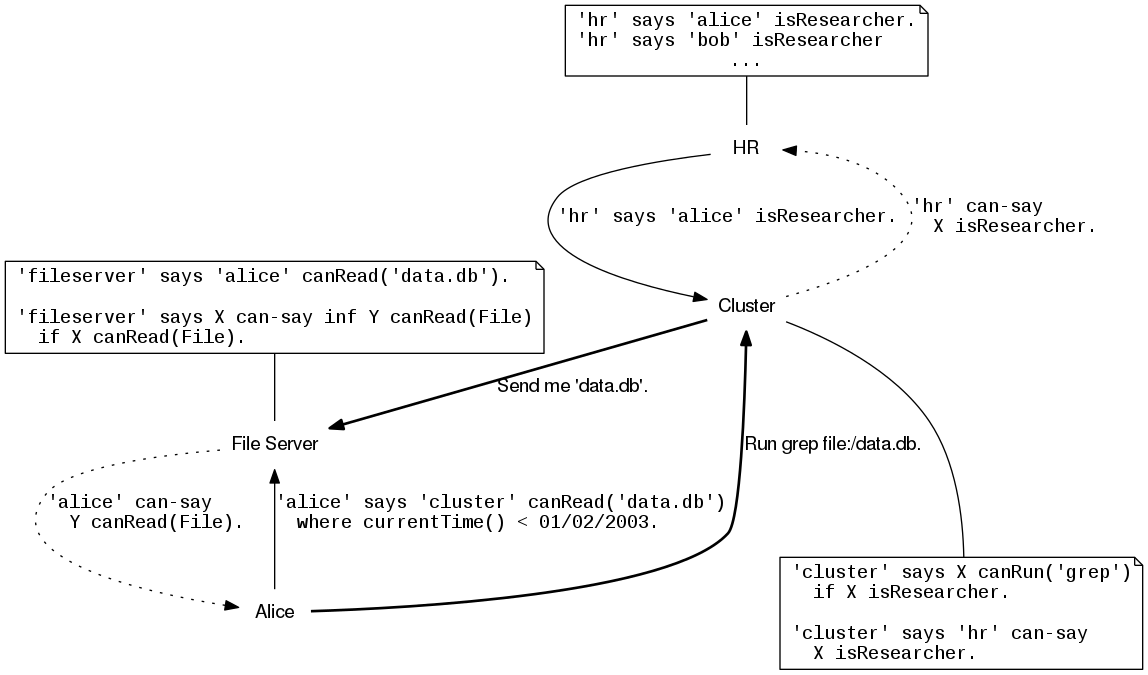
\includegraphics[width=\textwidth]{figures/secpal-example.png}
  \caption[Example of delegation on a cluster.]{Example of delegation when running a command on a cluster.  Bold links show requests, plain links show the sending of SecPAL statements, and dotted links indicate delegation relationships.  SecPAL assertions at each location are shown in notes.}
  \label{fig:delegation-example}
\end{figure}

Alice requests the cluster run a search on her data.  Her data is on the file-server.
The cluster has a SecPAL policy that only researchers can run the search:
It also has a rule that says the human resources department (HR) can say who is a researcher.
\begin{lstlisting}
'cluster' says X canRun('grep')
  if X isResearcher.

'cluster' says 'hr' can-say
  X isResearcher.
\end{lstlisting}
The cluster queries HR if Alice is a researcher. HR responds by saying she is.
\begin{lstlisting}
'hr' says 'alice' isResearcher.
\end{lstlisting}
The cluster does not know how HR knows that Alice is a researcher. But it
is content \emph{to trust} HR's assertion that she is.  HR may have a SecPAL
instance and policy of their own to make this decision and send it to the
cluster. Alternatively they might be using a conventional database.  Provided
they give this SecPAL assertion to the cluster, it does not care
how they came by it.  The one limitation the cluster has is that it
\emph{must} be HR telling them. HR cannot delegate the decision
further.

The cluster is now convinced that Alice may run the search.
It requests the database from the file server.  The file
server knows that Alice can read her data and that anyone who can read
a file may say who else can read it.
\begin{lstlisting}
'fileserver' says 'alice' canRead('data.db').
'fileserver' says X can-say inf Y canRead(File)
  if X canRead(File).
\end{lstlisting}
Using SecPAL, the file server determines that Alice can say who
reads her data.  Alice gives the file server a statement that
the cluster can read her file (for a short time
period).
\begin{lstlisting}
'alice says 'cluster' canRead('data.db')
  where currentTime() < 01/02/2003.
\end{lstlisting}
The file server gives the cluster the data.
The cluster runs the search and hands the results back to Alice.

\begin{figure}
  \centering
  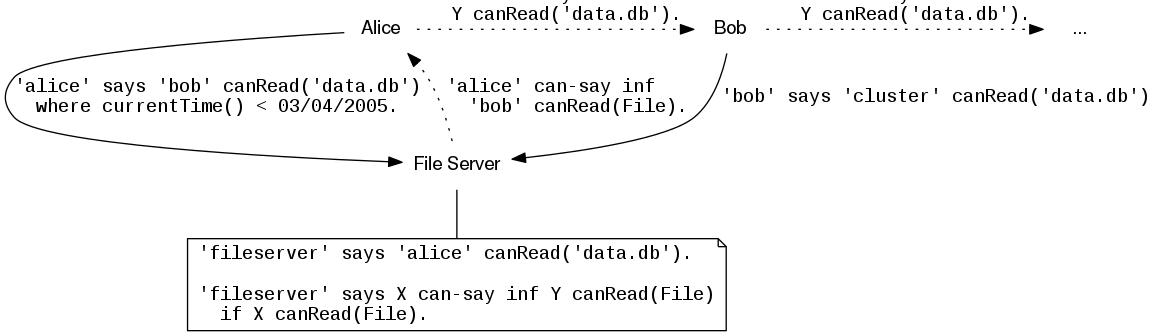
\includegraphics[width=\textwidth]{figures/secpal-example-delegation.png}
  \caption{Example of unbounded delegation.}
  \label{fig:unbounded-example}
\end{figure}

This simple example shows how different principals can make decisions using delegation mechanisms.
SecPAL allows for more complicated delegation relationships, however. 
The file server gave Alice the ability to delegate who could read her file by using the \texttt{can-say inf} verb.
Alice might allow Bob to share her data set with others who might also be allowed to share it for a limited time (\autoref{fig:unbounded-example}).

\begin{figure}
  \centering
  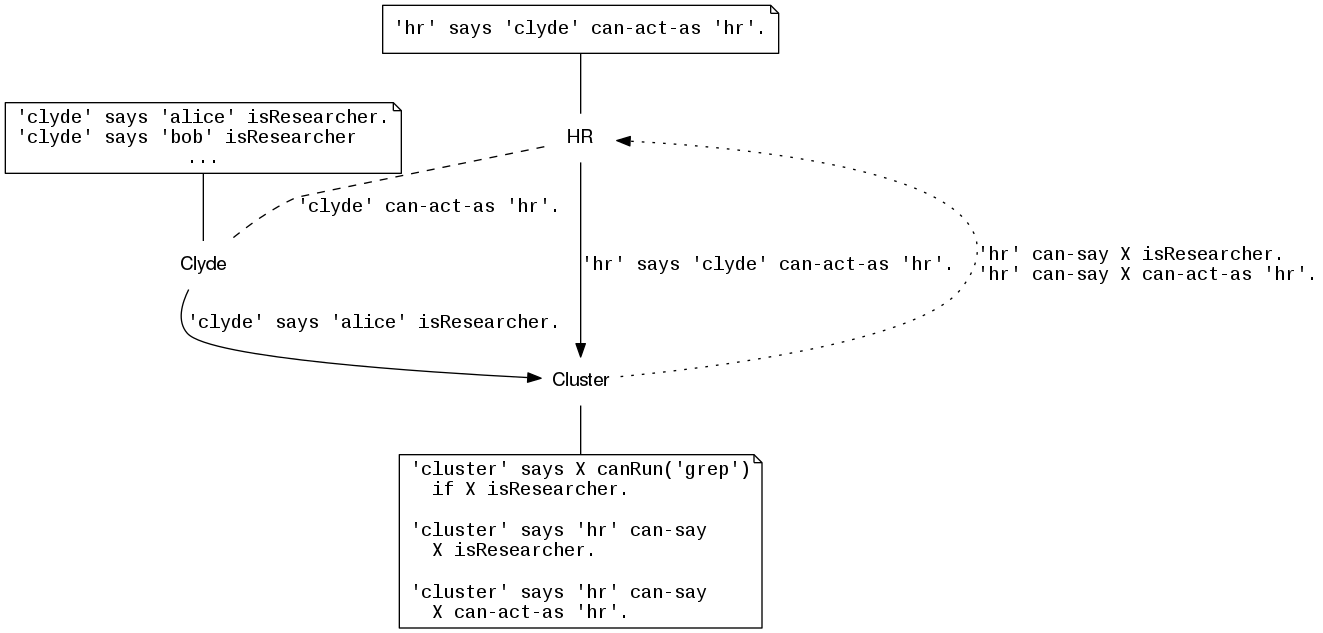
\includegraphics[width=\textwidth]{figures/secpal-example-roles.png}
  \caption[Example of delegation with roles.]{Example of delegation with roles.  Role relationships are shown with dashed links.}
  \label{fig:roles-example}
\end{figure}

An alternative to asking to the HR server directly if Alice is a researcher is
to use roles (shown in \autoref{fig:roles-example}). Many people work in HR. The
cluster might accept the word of any of them. To do this the cluster delegates
to HR to name anyone who \emph{acts as} HR. Suppose that HR responds that Clyde
can act for them.
\begin{lstlisting}
'cluster' says 'hr' can-say
  X can-act-as 'hr'.

'hr' says 'clyde' can-act-as 'hr'.
\end{lstlisting} Now, on the cluster, Clyde's word is as good as HR's. Clyde
sends the necessary facts about Alice. The policy check now runs as before. Note
that the restrictions on HR also apply to Clyde: he still cannot delegate the
decision further. Clyde may have more capabilities than HR if there are other
provable assertions about him. The \emph{can-act-as} means that Clydes is at
least as powerful as HR: he inherits HR's capabilities.

\begin{figure}
  \centering
  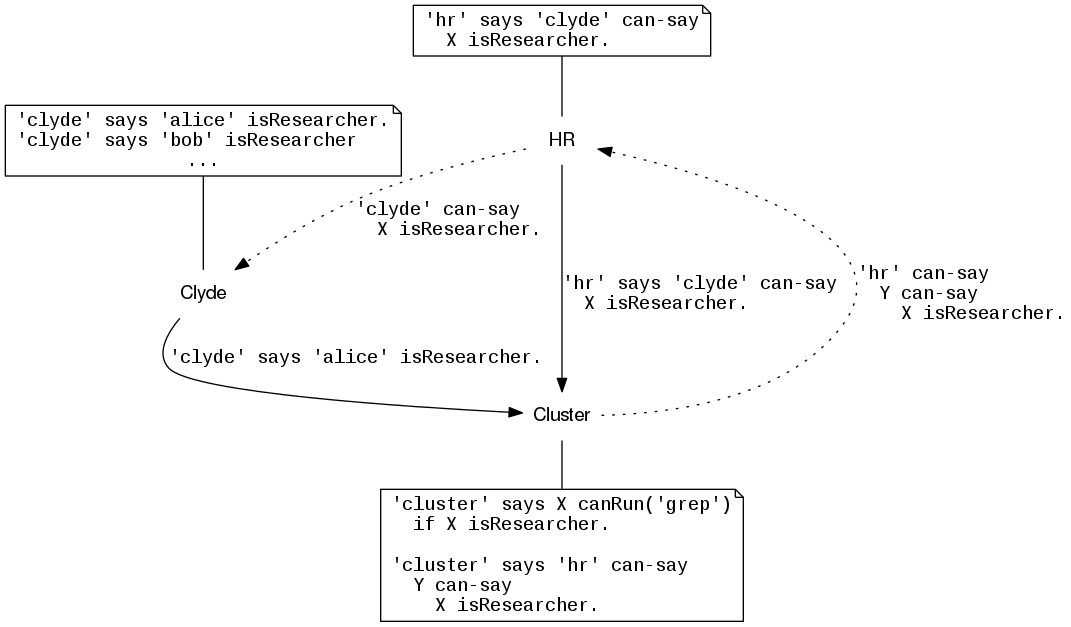
\includegraphics[width=\textwidth]{figures/secpal-example-delegation2.png}
  \caption{Example of depth bounded delegation.}
  \label{fig:depth-example}
\end{figure}

Depth-bounded delegation with the \emph{can-say} statement is an alternative to
roles (\autoref{fig:depth-example}). Instead of letting HR state who is a
researcher to HR, the cluster lets HR \emph{decide who decides}. HR delegates to
Clyde and the process continues as before. Depth-bounded delegation allows
delegation statements to be chained to an arbitrary (but finite) depth, without
allowing for unbounded delegation. It is preferable to roles as it allows HR to
delegate some but not all decisions to others. If role assignment is used then,
on the cluster, anywhere \texttt{'hr'} follows the \texttt{says} in an
assertion, then it can be replaced with \texttt{'clyde'}: they are the same.

SecPAL's delegation mechanisms can describe many different relationships. Yet it
remains conceptually and semantically simple. This power makes SecPAL attractive
for situations where entities are distributed and there is no central decision
point, as we can capture the trust relationships between entities and at
different places. This makes SecPAL a very appropriate language to model the
policies of the mobile ecosystem, as every device, user, company and store has
their own policies and makes there own decisions, sometimes by talking to each
other. We will discuss our reasons for using SecPAL to capture the policies of
the mobile ecosystem further in \autoref{chap:apppal}, but to sumarise its
ability to delegate and capture policies makes it a good starting point.


\section{Policy Languages}
\begin{figure}
  \centering\sffamily\scriptsize
  \begin{chronology}[5]{1987}{2017}{\textwidth}
    \event{1988}{X.509}
    \event{1991}{A Calculus for Access Control~\cite{abadi_calculus_1991}}
    \event{1994}{Authentication in the Taos OS~\cite{wobber_authentication_1994}}
    \event{1996}{PolicyMaker~\cite{blaze_decentralized_1996}}
    \event{1998}{KeyNote~\cite{blaze_keynote:_1998}}
    \event{1999}{SPKI/SDSI\cite{ellison_spki_1999}}
    \event{2000}{Delegation Logic~\cite{li_practically_2000}}
    \event{2001}{Ponder~\cite{damianou_ponder_2001}, XACML}
    \event{2002}{RT~\cite{li_design_2002}, Binder~\cite{detreville_binder_2002}}
    \event{2004}{Cassandra~\cite{becker_cassandra:_2004}}
    \event{2005}{XACML 2.0}
    \event{2006}{SecPAL~\cite{becker_secpal:_2006}}
    \event{2008}{DKAL~\cite{gurevich_dkal:_2008}}
    \event{2009}{DKAL2~\cite{yuri_gurevich_dkal2---simplified_2009}, Ponder2~\cite{twidle_ponder2:_2009}, SecPAL4P~\cite{becker_framework_2009}}
    \event{2010}{XACML 3.0~\cite{oasis_extensible_2013}}
    \event{2011}{SecPAL4DSA~\cite{aziz_secpal4dsa:_2011}}
    \event{2013}{DKAL$\star$~\cite{jeannin_dkal*:_2013}}
    \event{2016}{AppPAL~\cite{hallett_apppal_2016}}
  \end{chronology}
  \caption{Timeline of the development of different policy languages.}
  \label{fig:policy-language-chronology}
\end{figure}


We have introduced SecPAL to describe policies, and will study it further in the
rest of the thesis to describe the policies of the mobile ecosystem. In this
section we give a survey of some other influential policy languages. A timeline
of the development of the languages mentioned here is shown in
\autoref{fig:policy-language-chronology}.

\paragraph*{PolicyMaker.}
PolicyMaker~\cite{blaze_decentralized_1996} is a language for permitted actions.
It grew out of the logics of authentication of Wobber, Abadi, Burrows and
Lampson~\cite{wobber_authentication_1994,abadi_calculus_1991}; as well as a
dissatisfaction with identification mechanisms such as X.509 and PGP
certificates. These mechanisms identified users but could not link them to what they could do.

To describe the authorizations, assertions hold trust information.
Many assertions form a policy. An assertion has a source (either
the local policy document or a public key). The source \emph{asserts} that the holder of a key
(or more complex arrangements such as three of four keys) can do any action that matches the \emph{filter}. The filter itself is
an arbitrary program that can make a yes/no decision.
Blaze~\etal~give examples using regular expressions and a reduced version of
AWK~\cite{aho_awk-pattern_1979}. They note, however, that
any programming language could be used. The device policy can be queried by a
key holder \emph{requesting} a given action.

Blaze~\etal~give an example of this scheme being used as part of an email
server. A user, Alice, identified by key \texttt{0x12345678} can
send emails with the from header set to Alice and the organization set to Bob
Labs.

PolicyMaker is installed on a server. It receives queries and gives answers.
The policy is on the server is:

\begin{lstlisting}
policy ASSERTS
  pgp:'0x12345678'
  WHERE PREDICATE=regexp:'(From: Alice) &&
    (Organization: Bob Labs)';
\end{lstlisting}

When Alice sends an email using a PolicyMaker enhanced SMTP
client she signs her message with her key.  The mail server
checks the signature and queries the policy server with her message:

\begin{lstlisting}
  pgp:'0x12345678'
  REQUESTS  'From: Alice
             Organization: Bob Labs

             Hello World!';
\end{lstlisting}

If Alice's message is okay then the SMTP server will send it.  If it does not match the policy then it will not.

\paragraph*{KeyNote.}
PolicyMaker is the basis for KeyNote~\cite{blaze_role_1999,blaze_keynote:_1998}.
KeyNote simplifies the arbitrary filter languages, offering instead one based on
C that always returns a boolean answer. KeyNote allows the policy server to do
the signature verification instead of the querying application. It also makes the
syntax more readable. KeyNote also trades PolicyMaker's generality for a more
realistic scenario using public-key infrastructure. The prior policy for KeyNote
could be written:

\begin{lstlisting}
Authorizer: "POLICY"
Licensees: "RSA:abc123"

KeyNote-Version: "2"
Local-Constants: Alice="RSA:12345678" 
Authorizer: "RSA:abc123"
Conditions: (app_domain == "RFC822-EMAIL") &&
    (name="Alice") &&
    (organization="Bob Labs");
\end{lstlisting}

Checking whether a PolicyMaker or KeyNote policy is satisfied is
NP-hard~\cite{blaze_compliance_1998}. PolicyMaker assertions can involve
arbitrary programs written in Turing complete languages. Blaze~\etal{} restrict
these programs to those that run in polynomial time for all inputs pertinent to
a request.

A weakness of these languages is that they cannot express relationships among
users. You cannot have policy where the subject is a set of users. The example
policy could not be written as \emph{anyone working in R\&D can send email from
Bob Labs.}

%\subsection{SPKI/SDSI}

\paragraph*{SPKI/SDSI.}
Unlike PolicyMaker, SPKI/SDSI~\cite{ellison_spki_1999} was
designed to associate keys with roles.  A user, Alice with key~$K_A$,
can present a certificate that says she \textbf{can act as} (a role assignment) a \emph{Bob Labs
employee} (authorized by Bob with key~$K_B$) for one~year.

\begin{equation*}
  (K_A,~\text{\tt BobLabsEmployee},~K_B,~1~\text{year})
\end{equation*}

Bob can also create authorization certificates to let his employees
to send emails. Optionally they can delegate the decision further.

\begin{equation*}
 (K_B,~(K_B,~\text{\tt BobLabsEmployee}),~\bot,~\text{\ttfamily send\_email},~1~\text{year})
\end{equation*}

PolicyMaker checks whether to allow a specific user's action. SPKI/SDSI associates users with roles and
roles with tasks. The SPKI/SDSI version of the email sending policy (shown above) does not
specify that all emails sent by Employees must have a field listing the lab as
the sending organization. That part of the policy must be added by
whatever implements the \texttt{send\_email} functionality. One of the
advantages of SPKI/SDSI is that it allows a higher-level view of the policy by
associating groups of users with a role, and roles with allowed actions.

SPKI/SDSI does not have a formal semantics.  The language's precise meaning must be inferred from
RFC 2693, which loosely defines it in English~\cite{ellison_spki_1999}. There are
several later attempts at fitting semantics to the
language~\cite{joseph_y._halpern_logic_1999,abadi_sdsis_1998,howell_formal_2000,dwaine_clarke_certificate_2001}.
Not all covered every aspect of SPKI/SDSI's features, however. No definitive standard has appeared.

\paragraph*{RT.}
The focus on roles led to the RT family of
languages~\cite{ninghui_li_design_2002}. RT associates policy
decisions with roles. This is similar to how \ac{RBAC} systems associate access
decisions to the roles a user holds.  Policies are expressed as Horn
clauses.  A rule such as:

\begin{lstlisting}[language=prolog]
Bob.employee :- alice.
Bob.employee.sendEmail :- Bob.employee.
\end{lstlisting}

\noindent Is read as \emph{Bob says Alice is an employee, and Bob says an
employee can send emails if they are an employee.}  Li~\etal{}
describe many different variants of RT with various features.  The most basic variant is
\RT{0}{}~\cite{li_distributed_2003}. \RT{1}{} adds support for
parameterized roles. \RT{2}{} adds logical objects on top of the
roles.  As well as these variants, the RT family of languages
supports optional feature sets: \RT{}{T} allows for policies with
thresholds (i.e. Alice can send an email if two out of three of the
board members approve it). \RT{}{C} adds constraints. Finally, \RT{}{D}
adds delegation~\cite{ninghui_li_design_2002}.

Unlike PolicyMaker, the RT family of languages is tractable. Li~\etal~prove a guarantee
that a query will be answered soundly in polynomial time in the size of the
policy. To give this guarantee, the researchers showed the languages could be
reduced to Datalog. Datalog is a database language with known complexity
guarantees and fast evaluation. It is similar Prolog. They also showed similar
languages, like Binder~\cite{detreville_binder_2002} and
Delegation~Logic~\cite{li_delegation_2003,li_practically_2000}, could be
described using Datalog as well.

Datalog is limited in that it cannot describe structured data. Consider a rule
that lets Alice send email between 9am and 5pm. We might want some function to
compare whether a time is within a range. In Datalog we cannot trivially write
this function. We would have to say for each possible time if it is in that
period. Generally, when there is data that has structure such as file paths,
times or numeric intervals: Datalog databases can become overly large.

To solve this Li~\etal{}~modified Datalog to create
Datalog\textsuperscript{C}~\cite{li_datalog_2003}. Datalog\textsuperscript{C} is
based on Constraint Datalog~\cite{revesz_constraint_1995,revesz_safe_1998} and
supports constraints whilst keeping Datalog's tractability. It focuses on the
constraints typical to a policy languages instead of those for database
programming.

Showing a policy language is translatable to Datalog\textsuperscript{C} allows
the language author to prove that evaluating policies in their language can be
done with the same time and space complexities as Datalog\textsuperscript{C}.
Datalog\textsuperscript{C} is used as a foundation for many other policy
languages including SecPAL as well as RT.

\paragraph*{Ponder.}
Ponder, like SecPAL, is a language for specifying policies for distributed
systems~\cite{damianou_ponder_2001}. Ponder supports positive and negative
authorization, delegation, obligation, roles and constraints. It uses
constraints to extract the attributes of principals, read state, and deal with
time. A policy that trainee engineers are not allowed to send emails could be
written:

\begin{lstlisting}
inst auth- engineersCanEmail {
  subject e =/Engineer;
  target  /mail_server;
  action send_email();
  when e.status() == ``trainee'';
}
\end{lstlisting}

Since Ponder allows positive and negative policies, conflicts can occur. Ponder
does not resolve the conflicts itself. Instead it detects them using static
analysis and reports them to the policy author as bugs in the policy
specification. Ponder2~\cite{twidle_ponder2:_2009} simplified Ponder and added
policies for decentralized environments. Ponder2 also provides a control
language called \emph{PonderTalk}, which lets the decision engine send messages
to the objects it manages.

\paragraph*{Cassandra.}
Cassandra is a trust management language to model large systems.
It was demonstrated on the NHS Spine: a system to let healthcare
workers share patient
data~\cite{becker_cassandra:_2004,becker_cassandra:_2004-1}.  The
language is similar to RT, using both a Datalog\textsuperscript{C} and some
of its syntax. Cassandra, however, focuses on roles instead of general access
control mechanisms.  Principals \emph{activate} roles when they need to act in its
capacity.  This lets one principal hold different roles, with
different capabilities, at different times and at different
locations.  A \emph{hospital} \emph{admin} might allow a
\emph{clinician} access to a \emph{patient}'s records if they
have the role of \emph{Clinician} at the hospital, and can
\emph{activate} the role of \emph{Treating Clinician} for that patient
at this \emph{hospital}:

\begin{lstlisting}
hospital@admin.permits(clinician, Read-Records(patient)) <-
  hospital@hasActivated(clinician, Clinician(hospital)),
  hospital@canActivate(clinician, TreatingClinician(hospital, patient))
\end{lstlisting}

Cassandra allows for powerful control of different roles, and enables
delegation by allowing third-parties to activate and remove roles
on others.  
Becker worked on Cassandra for his doctorate.  He went on to work on SecPAL.

\paragraph*{SecPAL Extensions.}
We started this chapter, by describing SecPAL. Since SecPAL was first described
various tweaks and extensions were made to the language. SecPAL was extended to
allow existential queries. This allowed it to answer
queries such as \emph{``does Alice say Bob can read any of her files?''} or
\emph{``do all Alice's apps meet her installation policy?''}, which could only
be answered by manually making multiple queries before. 
%
Becker also described the possibility of dynamic assertion retrieval, which
would allow SecPAL to fetch and add assertions to it's assertion context when
making queries. In the case of delegation this would allow a delegated
principals assertions to be imported dynamically rather than having to be
present in the AC before evaluating a query. Becker defined a safety condition,
but didn't describe a protocol for retrieving assertions,
however~\cite{moritz_y_becker_secpal:_2009}.

Becker also noted that roles and the \emph{can-act-as} statement had proven to
be of limited use. Delegation using \emph{can-say} could replace it with greater
control in all cases Wherever that \emph{can-act-as} to use exclusively depth
bounded delegation (as we showed in \autoref{ssec:delegation_in_secpal}). 

\section{Moving Forward}

This chapter described SecPAL, and a number of other policy languages designed
in the same time frame. In the next chapter we show how we took SecPAL and
instantiated it to describe the policies surrounding mobile devices. In doing so
we created AppPAL. We describe the language and our implementation of it in
\autoref{chap:apppal}.

AppPAL fits into this background of policy languages by extending SecPAL. It
does not have new semantic language features to describe new kinds of policies.
Instead its novelty lies in the application to a domain that has not before had
its policies captured using a precise language.

\end{document}

%%% Local Variables:
%%% mode: latex
%%% TeX-master: "../ch2"
%%% End:
